\section{System Evaluation}
\label{chap:5}

In this section explains the details of the system evaluation. The randomised distributed algorithm proposed in \cite{yves2009optimal} was tested with three synchronisation techniques explained in section \ref{chap:3} using the simulator previously described in section \ref{chap:4}. The model for generating random graphs for the networks topologies are described in this section. The evaluation metrics, hardware and software used for testing and the simulation workflow are also part of this section.   

% The theoretical bound for this algorithm is known to be $O(\log N)$. The synchronizers time and message complexity were discussed in section \ref{chap:3}. 

\subsection{Evaluation Criteria}



The metrics used to measure the algorithm are time and messages complexity. The way to measure the time complexity in the synchronous model is counting the number of rounds until an algorithm terminates. Message complexity consists of counting the total number of messages sent by the processes per round.

The primary goal of the simulation is to empirically evaluate the time complexity of the \textit{MIS} algorithm and the message overhead on synchronous systems using different synchronisation techniques. The secondary goal is to examine how the properties of the topologies progressively change in each round of the \textbf{MIS} algorithm.


\subsection{Network Models}
\label{sec:topology}


The network topologies need to be generated before testing the \textit{MIS} algorithm. Topologies represent the distributed system in which the algorithm is going to run. There is a mapping from vertices of the graph to processors and from edges to the communication channels.  The Stochastic Block Model \textbf{SBM}, proposed in \cite{holland1983stochastic},  is a model used to generate random graphs. This model is a generalisation of the Erd\~os--R\'enyi model, and it was used to produce the topologies for the simulations. 

Before entering in details with the \textbf{SBM}, a brief explanation about the Erd\~os--R\'enyi model is presented. This model for random graphs, proposed in \cite{erdds1959random}, has two variants. The one used in this project is the $G(n, p)$ model in which a graph is constructed by connecting $n$ vertices randomly. An edge is included in the graph between two vertices $i,j$ with independent probability $p$. On \cite{erdos1960evolution} Erd\~os and R\'enyi presented some important properties about the connectivity of the generated graphs. A summary of these properties is cited below.


\begin{enumerate}
\item If $p<{\tfrac {(1-\epsilon )\ln n}{n}}$, then the graph $G(n, p)$ it is very likely to be disconnected.
\item If $p>{\tfrac {(1+\epsilon )\ln n}{n}}$ , then the graph $G(n, p)$ it is very likely to be connected.
\end{enumerate}

In conclusion, in the event that connected graphs are needed, then ${\tfrac {\ln n}{n}}$ is the threshold of $p$, for which the generated graphs $G(n, p)$ will almost surely be connected.  

In the \textbf{SBM}, the networks are characterised by blocks structures; these groups or blocks define a partition of the network. Each vertex is associated with a group, and the probability of an edge between two vertices depends on the group of the vertices. It is possible to obtain graphs that are denser in some regions adjusting the probabilities of the groups. The probability for each group is defined in a probability matrix. In the next section, a formal definition of the \textit{SBM} is given with some examples of graphs generated by this model.


\subsection{Stochastic Block Model}

The \textbf{SBM} can be considered a probabilistic or generative model in which a probability is assigned to each pair of vertices $i,j$ in the network. This model defines a probability distribution over the network $Pr(G | \theta)$, where $\theta$ is a set of parameters that define the graph. For a given $\theta$, it is possible to generate a network instance G by flipping a coin between every possible pair of vertices of the $G$ according to the probability distribution. 

The Stochastic Block Model is formally defined by: 
\begin{enumerate}

    \item $k$: a scalar representing the number of blocks groups, clusters or modules in the network.
    \item $\overrightarrow{z}$: a vector of n element where $z(l)$ gives the block index of the vertex $l$.
    \item $M$ is a $k * k$ stochastic block matrix, where $M_{ij}$ gives the probability that a vertex of block type $i$ is connected to a vertex of block type $j$.
\end{enumerate}



The edges in the graph generated by the SBM are not necessarily identically distributed, and the existence of two edges are independent. A large number of parameters allows the \textbf{SBM} to produce very different structures. If $M_{ij} = p$ for each pair of blocks, then the \textbf{SBM} is reduced to the Erd\~os--R\'enyi model of random graph $G(n,p)$. The figure \ref{fig:erdos} show an example of stochastic block matrix in which every probability is the same for $k = 3$ blocks. Note that this is a square matrix and $k$ should be defined before $z$ and $M$. The probability distribution is the same for each block, as a consequence, the graph looks like one component even if the vertex belongs to different blocks types.

 The figure \ref{fig:sbm} is another example of a random graph. In this case, the probability distribution differs among blocks, and it is easier to visualise the different groups in the figure. The value $M_{i,j}$ where $i = j$ represent the probability of one edge between two vertices in the same group and the entry $M_{i,j}$ where $i \neq j$ represent the probability of one edge between two vertices in the different groups. 

When $M_{i,i}$ is greater than $M_{i,j}$ for $i \neq j$ the vertices tend to connect other vertices that are in the same group. For this configuration, the values of the diagonal are larger than values out of it. In this case, the communities are \textbf{assortative} and the edges are more common within the blocks. On the contrary, if $M_{ii} <  M_{ij}$ for $i \neq j$, edges between vertex of different communities are more common and the grouping is \textbf{disassortative}.


Many other grouping criteria and variation of \textit{SBM} exist in the literature \cite{carrington2005models,holland1983stochastic,airoldi2008mixed}. Particularly, for this project, the assortative grouping is used for generating topologies. The ${\tfrac {\ln n}{n}}$ threshold is used to set the probability of the diagonal in the block matrix of probabilities. 

\begin{figure}[ht]
\centering
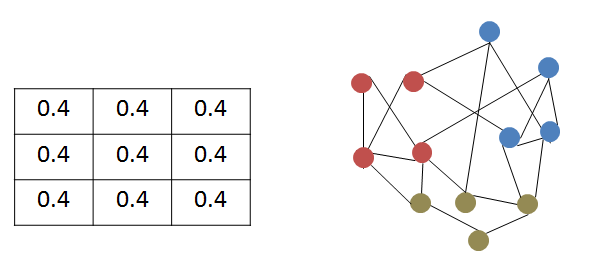
\includegraphics[width=1 \linewidth, height=5cm]{Erdos-Renyi.PNG} 
\caption{Example of SBM with equal probabilities}
\label{fig:erdos}
\end{figure}

\begin{figure}[ht]
\centering
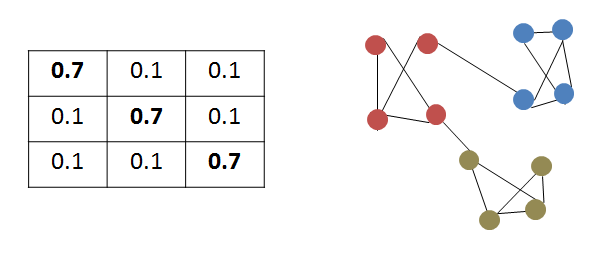
\includegraphics[width=1 \linewidth, height=5cm]{sbm.PNG} 
\caption{Example of SBM with assortative communities}
\label{fig:sbm}
\end{figure}

\subsection{Description of Experiments}

As mention in section \ref{chap:4}, the simulator was implemented in Elixir 1.3. The topology generator is a modified open source software written in Python under MIT license. Some modifications were done to the generator to adapt to the requirements. For instance, iterate only for the upper triangular adjacency matrix of the graph, modified the parameters, customised the file format to store the topologies and some other minors modifications.

The tests were run in a computer with processor Intel(R) Core(TM) i5--4210U of 1.7 and 2.4 GHz and RAM of 8 GB with additional 8 GB of SWAP. The operating system was a Linux 64 bit Debian base.


The value for $p$ was chosen to make sure that the generated graphs are connected in the Erd\~os--R\'enyi and \textit{SBM} model. Note that the algorithm for \textit{MIS} does not require this condition because it still finds the solution for a disconnected graph. However, the Beta Synchronizer construct a rooted spanning tree over the topology to perform the synchronisation, so if the topology is not connected the rooted spanning tree can not be constructed. In order to maintain the same topologies for all synchronizers, all the generated graphs were connected.  

The steps to perform the experiments are enumerated below:

\begin{enumerate}
\item Implementation of the synchronizers Alpha and Beta and Global.
\item Implementation of the Maximal Independent Set Algorithm using the global synchronizer.
\item Implementation of the Maximal Independent Set algorithm using the simulation Alpha and Beta.
\item Create the topology with the Stochastic Block Model according to the description in the section \ref{sec:topology}.
\item Run N times the synchronous algorithm for the \textit{MIS} and save the results for each synchronizer.
\item Compute the average and calculate the results.
\end{enumerate}



